\section{Model training and evaluation}\label{sec:evaluation}

In order to avoid over-fitting and be able to evaluate our model on a real-world scenario, the dataset has to be initially split into a \emph{training set} and a \emph{testing set}.
Consequently, every kind of consideration, analysis and training was made by using the training set only, to avoid information leaking from the testing set to the training set.
A final testing can be done at the very last stage, once we are satisfied with the trained model and we are willing to test it against never seen data (see next section).

A powerful tool that can help us understand how to properly choose the features, the regressor and its parameters, and effectively evaluate the model before the final testing, is the \emph{cross-validation}, explained in the following.

\subsection{Metrics}\label{sec:metrics}

In regression theory, there are two possible metrics that can be used to assess the accuracy of a regressor, which are different from the metrics used in classification theory, since the ground truth domain is continuous.

\paragraph{Mean Squared Error}
The MSE is a measure of the expected value of the quadratic error between each predicted value $y_i$ and its true value $\hat{y}_i$, therefore a lower value indicates a better accuracy.
Given $N$ as the number of samples, it is mathematically computed as follows:

\[
	\text{MSE}(y, \hat{y}) = \frac{1}{N} \sum_{i=1}^{N} (y_i - \hat{y}_i)^2
	\qquad [0, \infty)
\]

Since it is a scale-dependent metric, it is important to contextualize it into the scale of reference (i.e. a MSE of 0.2 is worse in a domain ranging from 1 to 10 than in one ranging from 1 to 100).

\paragraph{$R^2$-score}
The coefficient of determination is a measure of how well unseen samples are likely to be predicted by the model, and it represents the ratio between the variance of the predicted values and the variance that would be predicted by the model.
Given $N$ as the number of samples, and $\bar{y}$ as the mean of the predicted values, it is mathematically computed as follows:

\[
	R^2(y, \hat{y}) = 1 - \frac{
		\sum_{i=1}^{N} (y_i - \hat{y}_i)^2
	}{
		\sum_{i=1}^{N} (y_i - \bar{y})^2
	} \qquad (-\infty, 1]
\]

It is a scale-invariant metric, therefore it is possible to compare $R^2$-scores across different domain ranges, however it is variance-dependent, so it might not be meaningful to compare it across different datasets.
A value of $1$ indicates that the regressor perfectly predicts the ground truth.
A value of $0$ indicates that the regressor always predicts the mean value $\bar{y}$, disregarding the input features.
A negative value indicates that the regressor behaves arbitrarily worse than predicting a constant.

\subsection{Cross-Validation}\label{sec:cross-validation}

It is a methodological error to evaluate metrics against the testing set and then use them to enhance the model, since this leaks information about the testing set which is supposed to be left unknown.
This phenomenon is known as \emph{over-fitting} and should be avoided.

One possible option to evaluate the model without using the testing set is to cut a separate sub-set from the training set, called \emph{validation set}, and compute the metrics against this one instead.
The drawback, however, is that this option further reduces the training set usable size.

A better approach consists in iteratively cutting a different small sub-set for validation from the training set, collect the metrics about each possible cut, and aggregate them in terms of mean and standard deviation (see figure~\ref{fig:kfolds}).
This way, the whole training set can be used.
This procedure is known as \emph{$k$-fold cross-validation}.

\begin{figure}
	\centering
	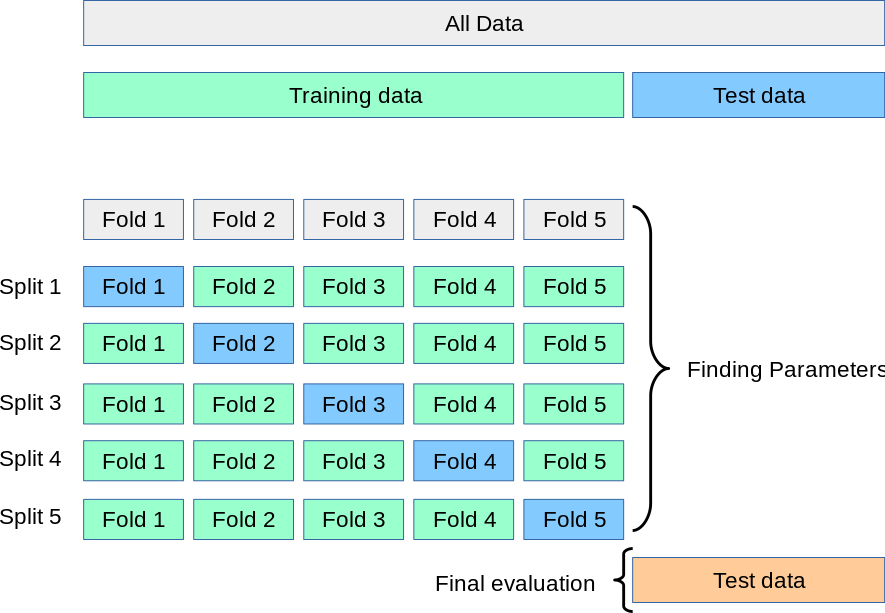
\includegraphics[width=0.5\linewidth]{assets/kfolds.png}
	\caption{$k$-fold cross-validation example with $k=5$ \cite{sklearn-crossval}}
	\label{fig:kfolds}
\end{figure}

The gathered metrics can effectively be used to evaluate the performance of the chosen regressors over the dataset.
At this point, it is possible to tune the regression model (i.e. by changing the free parameters of the regressors) without the risk of over-fitting (see figure~\ref{fig:grid-search-workflow}).

\begin{figure}
	\centering
	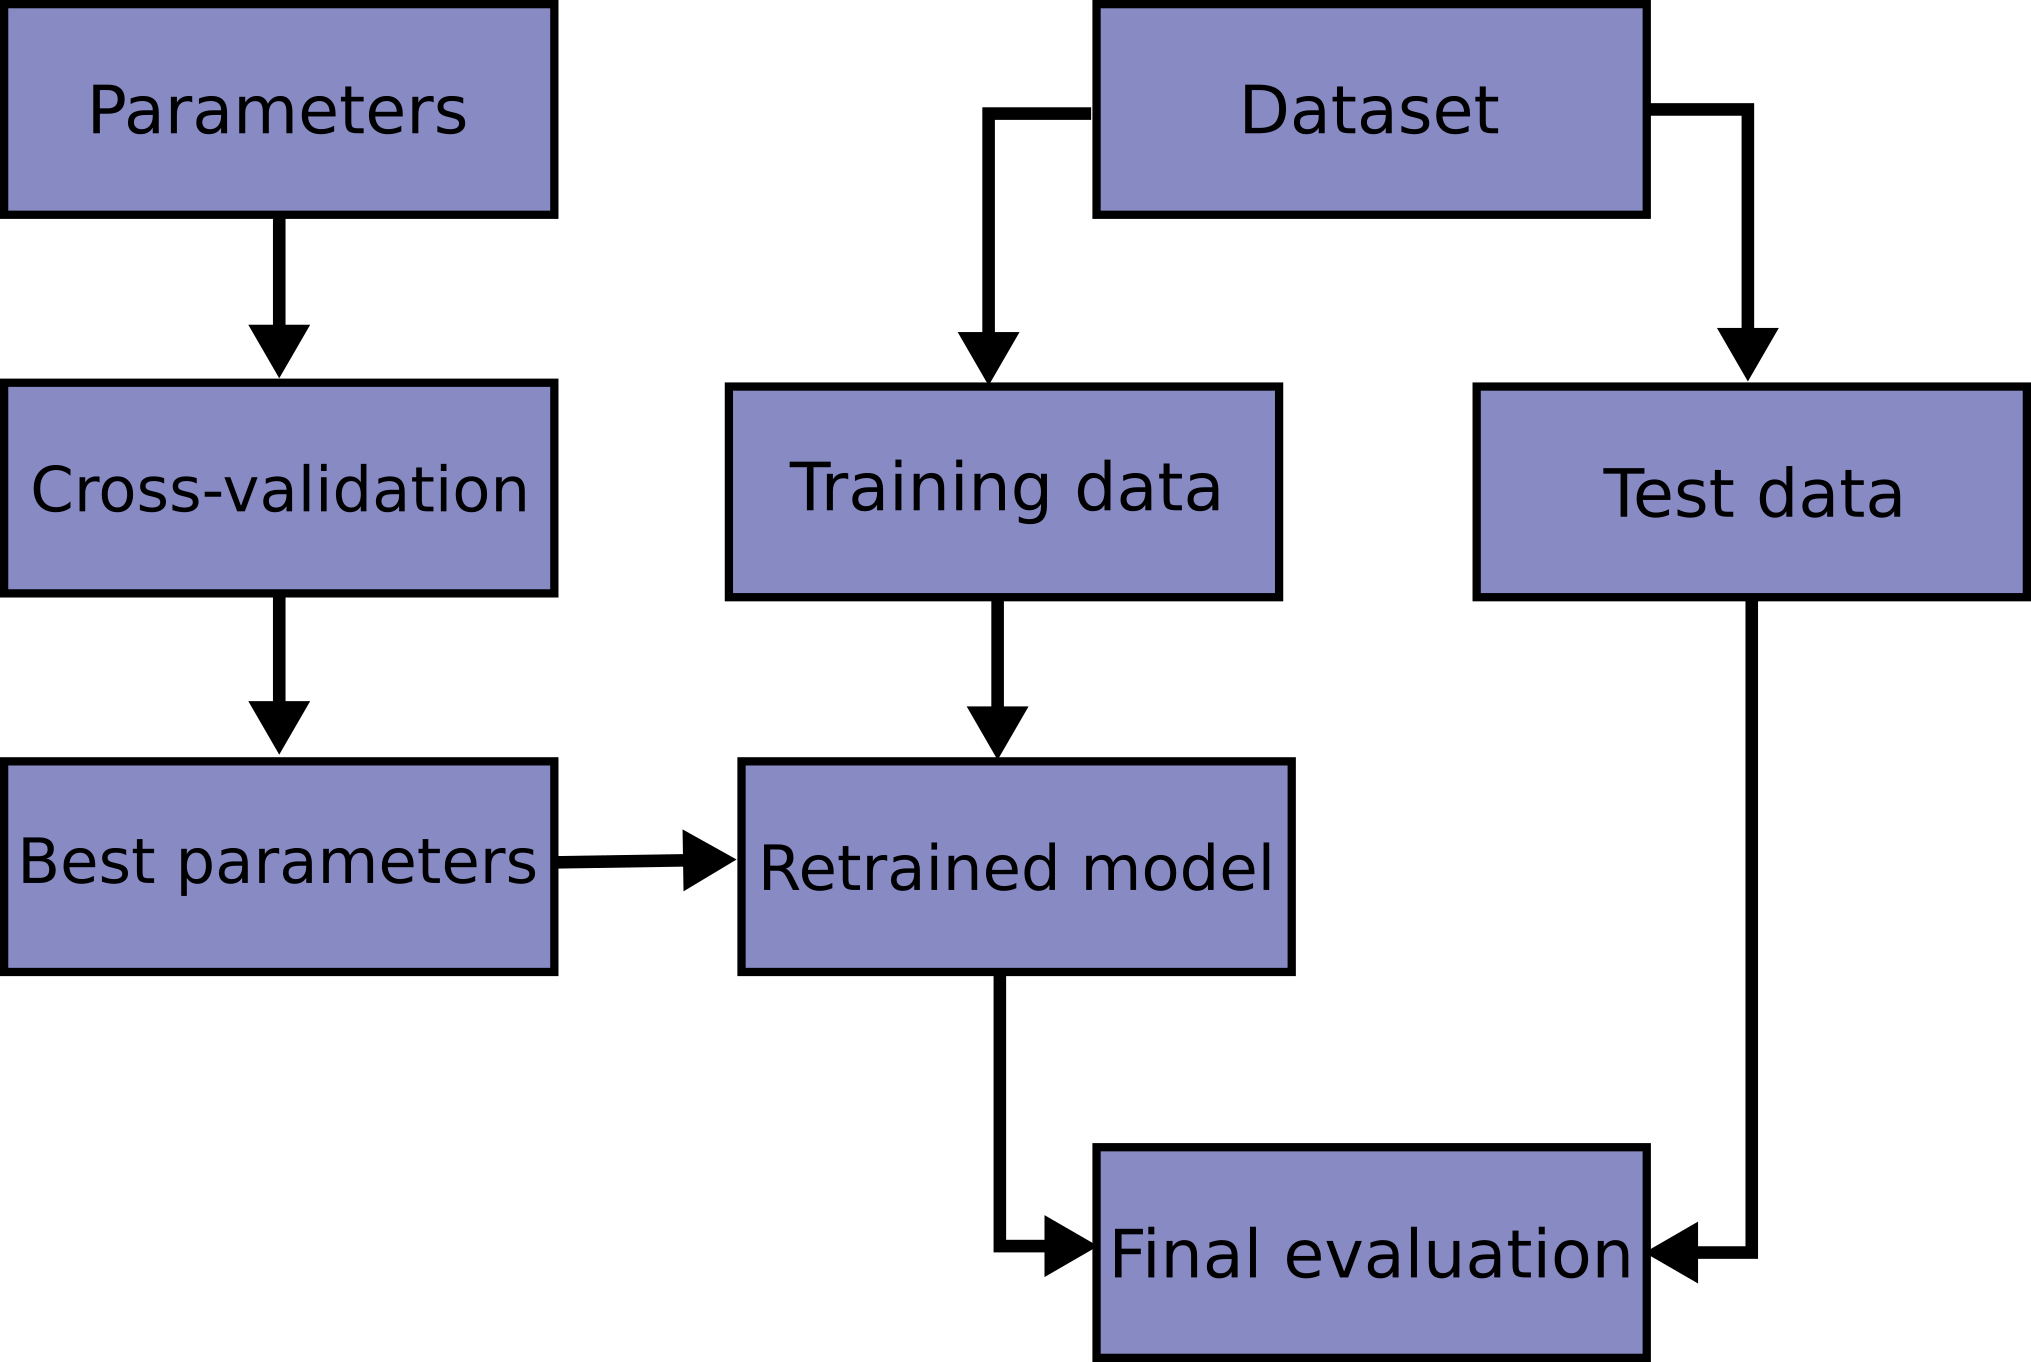
\includegraphics[width=0.5\linewidth]{assets/grid_search_workflow.png}
	\caption{Grid Search Workflow \cite{sklearn-crossval}}
	\label{fig:grid-search-workflow}
\end{figure}


\subsection{Enhancing the model}\label{sec:enhance-model}

The sklearn library provides a function \texttt{GridSearchCV()} for automatically selecting the best parameters for a given estimator, based on a grid of possible combinations.

At first, we computed the scores over a simple \texttt{LinearRegression} to evaluate the feature selection stage (see section~\ref{sec:features}).
Then we took advantage of the grid search to first optimize the linear model by using a Stochastic Gradient Descent regressor and a Ridge regressor with integrated cross-validation optimization.
We finally used again the grid search to find the suitable parameters (see section~\ref{sec:regression-??}) for $\nu$-SVM, $\epsilon$-SVM and KN-regressor.
For example, the best parameters found for the $\nu$-SVM regressor are reported in tables~\ref{table:cross-params-svr}.

\begin{table}
	\centering
	\begin{tabular}{lccc}
		\toprule
		& kernel & $C$ & $\nu$ \\
		\midrule
		valence mean & rbf & $10$ & $0.75$ \\
		valence std & rbf & $0.1$ & $0.25$ \\
		arousal mean & rbf & $1$ & $0.5$ \\
		arousal std & rbf & $0.1$ & $0.75$ \\
		\bottomrule
	\end{tabular}
	\caption{Best parameters for $\nu$-SVM regressor}
	\label{table:cross-params-svr}
\end{table}

%\begin{table}
%	\centering
%	\begin{tabular}{lcccc}
%		\toprule
%		& loss function & $\alpha$ & $\epsilon$ & tolerance \\
%		\midrule
%		valence mean & $\epsilon$-insensitive & $10^{-3}$ & $10^{-3}$ & $10^{-4}$ \\
%		valence std & $\epsilon$-insensitive & $10^{-2}$ & $10^{-2}$ & $10^{-4}$ \\
%		arousal mean & $\epsilon$-insensitive & $10^{-2}$ & $10^{-3}$ & $10^{-3}$ \\
%		arousal std & $\epsilon$-insensitive & $10^{-3}$ & $10^{-1}$ & $10^{-4}$ \\
%		\bottomrule
%	\end{tabular}
%	\caption{Best parameters for SGD regressor}
%	\label{table:cross-params-sgd}
%\end{table}

After refining the feature selection, we extracted the metrics of the best found estimators (see table~\ref{table:cross-scores}). It can be observed that, even after several attempts of feature selection (both manual and automatic), and optimization through cross-validation, no regressor could obtain a significant positive $R^2$-score for the values of ``valence std'' and ``arousal std'', and the obtained $R^2$-scores for ``valence mean'' and ``arousal mean'' were still quite low. This might be a consequence of the poor quality of the provided dataset, which required some preprocessing step on it that we didn't manage to accomplish.

\begin{table}
	\centering
	\begin{tabular}{lcccc}
		\toprule
		& valence mean & valence std & arousal mean & arousal std \\
		\midrule

		Linear & 0.44 ± 0.19 & -0.10 ± 0.12 & 0.39 ± 0.13 & -0.13 ± 0.18 \\
		SGD & 0.41 ± 0.25 & -0.11 ± 0.14 & 0.36 ± 0.19 & -0.16 ± 0.20 \\
		Ridge & 0.46 ± 0.16 & -0.04 ± 0.09 & 0.41 ± 0.14 & -0.10 ± 0.16 \\

		$\nu$-SVM & 0.40 ± 0.18 & 0.01 ± 0.06 & 0.48 ± 0.16 & 0.01 ± 0.07 \\
		$\epsilon$-SVM & 0.42 ± 0.18 & 0.02 ± 0.05 & 0.41 ± 0.13 & 0.01 ± 0.07 \\

		K-neighbors & 0.40 ± 0.08 & -0.06 ± 0.09 & 0.40 ± 0.16 & -0.07 ± 0.10 \\
		\bottomrule
	\end{tabular}
	\caption{Cross-validation $R^2$-scores with 95\,\% confidence intervals}
	\label{table:cross-scores}
\end{table}

However, a meaningful evaluation of the trained model can be still obtained by comparing the scores of the cross-validation against the scores obtained by the final testing stage.
This way, we can assess how worse the model will behave when we input never seen data (see section~\ref{sec:conclusions}).
In particular, given the results in table~\ref{table:cross-scores}, we decided to use Ridge, $\nu$-SVM and KN-regression as candidates for the final testing stage, as they seemed to be the best scoring regressors for each family of regression models considered.
